% =============================================================================
%  ILSC: Availability-Aware Semantic Cohesion for Microservice API Contracts
%  Draft for IEEE Access
%
%  COMPILING
%    latexmk -pdf ILSC_IEEE_Access.tex        (or: pdflatex, bibtex, pdflatex x2)
%
%  SUBMITTING TO IEEE ACCESS
%    This draft uses IEEEtran so that it compiles anywhere. To produce the
%    official IEEE Access layout:
%      1. Download the IEEE Access LaTeX template from the IEEE Author Center
%         and place ieeeaccess.cls beside this file.
%      2. Replace the \documentclass line below with:  \documentclass{ieeeaccess}
%      3. Uncomment the IEEE ACCESS FRONT MATTER block marked below and comment
%         out the IEEEtran front matter.
%    Nothing in the body needs to change.
% =============================================================================

\documentclass[journal]{IEEEtran}
% \documentclass{ieeeaccess}                    % <-- for the official submission

\usepackage{amsmath,amssymb,amsfonts}
\usepackage{booktabs}
\usepackage{graphicx}
\usepackage{multirow}
\usepackage{array}
\usepackage{url}
\usepackage{xcolor}
\usepackage{tikz}
\usetikzlibrary{arrows.meta,positioning,fit,backgrounds,calc,shapes.geometric}
\usepackage[caption=false,font=footnotesize]{subfig}
\usepackage{textcomp}
\usepackage{balance}

\graphicspath{{figs/}}

\newcommand{\ilsc}{\textsc{ilsc}}
\newcommand{\ilscm}{\ensuremath{\mathrm{ILSC}_{\mathrm{mean}}}}
\newcommand{\ilsct}{\ensuremath{\mathrm{ILSC}_{\tau}}}
\newcommand{\ilscn}{\ensuremath{\mathrm{ILSC}_{\mathrm{norm}}}}
\newcommand{\code}[1]{\texttt{\small #1}}

% consistent colours for the two TikZ figures
\definecolor{inkblue}{HTML}{2A4D8F}
\definecolor{inkred}{HTML}{A02F2A}
\definecolor{inkgreen}{HTML}{2B6252}
\definecolor{inkgrey}{HTML}{5A6473}

\begin{document}

% ------------------------------- FRONT MATTER (IEEEtran) ---------------------
\title{ILSC: Availability-Aware Semantic Cohesion\\
       Measurement for Microservice API Contracts}

\author{
  \IEEEauthorblockN{Author One, Author Two, and Author Three}
  \thanks{Manuscript submitted \today.}
  \thanks{The authors are with the Department of Computer Science,
          Institution, City, Country
          (e-mail: corresponding.author@institution.edu).}
  \thanks{The replication package, including both pinned corpus commits, all
          scripts, and every result artifact referenced in this paper, is
          available at \url{https://github.com/ANONYMOUS/ilsc}.}
}

% ------------------------- FRONT MATTER (IEEE ACCESS) ------------------------
% Uncomment this block and comment the IEEEtran block above when switching to
% ieeeaccess.cls.
%
% \history{Date of publication xxxx 00, 0000, date of current version xxxx 00,
%          0000.}
% \doi{10.1109/ACCESS.2026.DOI}
% \title{ILSC: Availability-Aware Semantic Cohesion Measurement for
%        Microservice API Contracts}
% \author{\uppercase{Author One}\authorrefmark{1},
%         \uppercase{Author Two}\authorrefmark{1}, and
%         \uppercase{Author Three}\authorrefmark{2}}
% \address[1]{Department of Computer Science, Institution, City, Country}
% \address[2]{Department, Institution, City, Country}
% \corresp{Corresponding author: Author One (e-mail: a.one@institution.edu).}
% \begin{abstract} ... \end{abstract}
% \begin{keywords} ... \end{keywords}
% \titlepgskip=-15pt

\maketitle

% =============================================================================
\begin{abstract}
Cohesion is a primary determinant of microservice design quality, yet it is
among the hardest properties to measure in practice: a microservice is defined
by its contract, deployed independently, and frequently owned by a team that
will not share its source. Existing measures either require runtime traces,
which are unavailable for third-party services and biased by the observation
window, or reduce cohesion to structural and lexical overlap that cannot
distinguish \code{Customer} from \code{Client}. We propose \ilsc{}
(Interface-Level Semantic Cohesion), a static metric computed entirely from an
API contract. \ilsc{} combines six similarity features---a sentence embedding of
a structured operation text, token overlap on names, paths and parameters,
domain-schema overlap, and a separate embedding of the description---under an
\emph{availability mask}: a feature contributes only when \emph{both} operations
of a pair carry it, and the weights redistribute over what remains, so a missing
field never counts as dissimilarity. This matters because specifications are
systematically incomplete: the mask is active on $73.6\%$ of within-service
operation pairs in our corpus and materially affects $68.4\%$ of services. We
evaluate on $2{,}206$ services ($97{,}912$ operations) curated from two pinned
sources, one of them a peer-reviewed corpus, and on two benchmark microservice
systems. Under controlled perturbation with a size-matched control, \ilsc{}
degrades monotonically for $20$ of $20$ services and degrades significantly
faster when injected operations come from a more distant provider (paired gap
negative for $20/20$, $p<10^{-6}$). Against code-level entity overlap, interface
similarity correlates at $\rho=0.41$ on hand-written specifications and
$\rho=0.49$ on specifications generated from source---a moderate, complementary
signal rather than a substitute for code analysis, and a $+0.08$ estimate of the
inflation that specification--code derivation introduces. Rankings are robust to
the weighting (Kendall's $W=0.99$ across $\pm40\%$ perturbations) and to the
threshold. We report three results that run against the metric. First, \ilsc{}
is strongly size-dependent ($\rho=-0.55$ with operation count), which no
null-model normalisation removes; we therefore publish quartile thresholds
stratified by size band, and show by regression over $1{,}570$ services that the
number of capabilities an author declares still predicts \ilsc{} once size and
publisher are controlled ($\beta=-0.017$, $p=0.006$). Second, on
\emph{generated} specifications the lexical baselines outperform \ilsc{}
(AUC $0.95$ versus $0.74$), because $81\%$ of a generated contract's schema
vocabulary is the code's own type vocabulary---specification provenance does not
merely inflate an interface-versus-code correlation, it inverts which metric
appears best. Third, \ilsc{} measures \emph{resource-level} rather than
\emph{capability-level} cohesion. On hand-written specifications, where the
comparison is not circular, \ilsc{} predicts code-level relatedness better than
both baselines (AUC $0.79$ versus $0.57$ and $0.65$).
\end{abstract}

\begin{IEEEkeywords}
Microservices, service cohesion, software metrics, API contracts, OpenAPI,
semantic similarity, sentence embeddings, software maintainability, static
analysis, threshold derivation.
\end{IEEEkeywords}

% =============================================================================
\section{Introduction}
\IEEEPARstart{C}{ohesion}---the degree to which the elements of a module belong
together---is one of the oldest design properties in software
engineering~\cite{stevens1974structured} and one of the least measurable in a
microservice architecture. A microservice is defined by its contract, deployed
independently, and frequently owned by a team that will not share its source
code~\cite{newman2021building}. The properties a maintainer most wants to know
are precisely the ones hardest to observe.

\subsection{The problem with existing approaches}
Existing approaches fail in three ways.

\textbf{They require runtime data.} Trace-based cohesion needs execution logs,
which are unavailable for third-party services, non-reproducible across
workloads, and contaminated by health checks. Worse, the absence of an operation
from a trace is not evidence that it is unused---only that it was not observed
in the window.

\textbf{They ignore meaning.} SIDC~\cite{perepletchikov2007coupling} counts
shared data types; LoCmsg~\cite{athanasopoulos2015cohesion} matches terms on
WSDL messages. Neither can see that \code{Customer} and \code{Client} name the
same concept, or that ``order'' (a purchase) and ``order'' (a sequence) do not.

\textbf{They assume complete inputs.} Real specifications are not complete. In
our corpus of $2{,}206$ public API descriptions, \code{operationId} is usable on
$88.4\%$ of operations, parameters on $90.7\%$, domain schemas on $78.7\%$, and
a description on only $73.0\%$. A metric that reads a missing description as
evidence of dissimilarity is measuring documentation quality and calling it
cohesion.

\subsection{The idea}
\ilsc{} scores each within-service operation pair on six features and averages
over all pairs. The contribution is not the feature set but the
\emph{availability mask}:
\begin{equation}
\mathrm{Sim}(O_i,O_j) \;=\;
\frac{\sum_k w_k \, m_{ijk} \, \mathrm{sim}_k(O_i,O_j)}
     {\sum_k w_k \, m_{ijk}},
\qquad
m_{ijk} \in \{0,1\}
\label{eq:mask-intro}
\end{equation}
where $m_{ijk}=1$ if and only if \emph{both} operations carry feature $k$. The
denominator is the weight actually available, not the total weight, so absence
is excluded from the comparison rather than counted against it.

Making that sound required a design constraint that is easy to miss: the feature
texts must be \emph{mutually disjoint}. An earlier version of this metric
included the description inside the embedded operation text \emph{and} scored it
separately, so deleting a description changed the embedding while the mask still
reported the embedding as available---the mask was defeated by its own inputs.
The texts are now disjoint and a regression test enforces it
(Section~\ref{sec:model-text}).

\subsection{What we found, including what we did not want to find}
The mask is justified by measurement, not assertion: it is active on $73.6\%$ of
within-service pairs and materially affects $68.4\%$ of services.

Perturbation behaves as the theory requires, \emph{against a control}. ``\ilsc{}
falls when you inject a foreign operation'' is close to tautological for a
mean-similarity score. The evidential content is the contrast: degradation
slopes order with semantic distance ($-0.035$ same-service, $-0.065$
same-provider, $-0.088$ cross-provider), and the paired gap is negative for
$20$ of $20$ services.

The correlation with code is moderate, and we reframe rather than overclaim:
$\rho=0.41$ on hand-written specifications, whose cluster-bootstrap interval
$[0.32,0.64]$ straddles the $0.4$ threshold we set in advance, because only two
of four benchmark services have any code-side variance.

Three findings run against the metric and are reported as such. \emph{(i)}
\ilsc{} is strongly size-dependent, and the null-model normalisation cannot
correct it; we publish size-stratified thresholds and separate the two effects
by regression. \emph{(ii)} On specifications generated from source code the
simplest lexical baseline wins, for a measurable reason. \emph{(iii)} \ilsc{}
measures resource-level cohesion, so a payroll service spanning ten unrelated
resources scores below services we labelled incohesive---and no reweighting
fixes this.

\subsection{Contributions}
\begin{enumerate}
\item \textbf{\ilsc{}}, a static interface-cohesion metric with an
      availability-aware weighting scheme, defined so that specification
      incompleteness is excluded from a comparison rather than penalised, and
      made sound by mutually disjoint feature texts
      (Section~\ref{sec:model}).
\item \textbf{A three-way validation without runtime ground truth}: controlled
      perturbation against a size-matched control, pair-level correlation
      against code-level entity overlap on two benchmark systems, and a
      head-to-head against two published baselines under an identical procedure
      (Section~\ref{sec:results}).
\item \textbf{Quartile thresholds over $2{,}206$ services}, derived as
      Bogner~et~al.~\cite{bogner2020rama} derive theirs, reported per source
      population \emph{and per size band}, together with the size dependence
      that makes the stratification necessary
      (Sections~\ref{sec:res-thresholds} and~\ref{sec:res-size}).
\item \textbf{A demonstration that specification provenance inverts metric
      rankings.} Evaluating interface-level metrics on specifications generated
      from source code makes the most superficial metric appear best. Because
      several widely used microservice benchmarks ship code-derived contracts,
      this is a methodological warning for the field and not only a fact about
      this study (Section~\ref{sec:res-4b}).
\item \textbf{A decision record whose rejections carry numbers}: keyword domain
      labelling rejected at $52\%$ agreement against a blind human sample, and
      LLM labelling rejected as circular with the metric under test.
\end{enumerate}

\subsection{Scope, stated once and kept}
\ilsc{} measures the semantic density of the operations a service
\emph{declares}. It is positioned as a \emph{proxy} for service cohesion, and
the validity of that proxy is the object of Experiment~3 rather than an
assumption. Everything the metric sees is in the contract; implementation
structure, runtime coupling and team ownership are out of scope by construction.
This is why the metric is not named ``service cohesion''.

% =============================================================================
\section{Related Work}
\label{sec:related}

\subsection{Cohesion metrics for service-oriented systems}
Cohesion as a design property originates with structured
design~\cite{stevens1974structured} and was formalised for object-oriented
systems by Chidamber and Kemerer~\cite{chidamber1994metrics} and unified by
Briand~et~al.~\cite{briand1998unified}, whose framework establishes the criteria
a cohesion measure should satisfy---non-negativity, monotonicity, and
insensitivity to the addition of unrelated elements outside the module.

Two service-era metrics are our direct baselines. \textbf{SIDC} (Service
Interface Data Cohesion)~\cite{perepletchikov2007coupling} measures the
proportion of operation pairs that share at least one data type.
\textbf{LoCmsg} (Lack of Cohesion in
messages)~\cite{athanasopoulos2015cohesion} measures the proportion of operation
pairs whose message terms are disjoint, and drives a decomposition procedure.
\textbf{WSIC}~\cite{hirzalla2009metrics} counts interface operations as a
flexibility proxy and is a size metric rather than a cohesion one. All three are
structural or lexical: they cannot recognise synonymy, and---critically for our
argument---none distinguishes a field that is \emph{absent} from a field that is
\emph{present and dissimilar}.

\subsection{Interface-level metric collection and thresholds}
Bogner~et~al.~\cite{bogner2017automatically} survey maintainability metrics for
service-based systems and find tool support scarce. Their
RAMA~\cite{bogner2020rama} closes part of that gap: a CLI that parses OpenAPI,
RAML and WADL, computes ten structural service metrics from the literature, and
derives quartile-based threshold bands (green/yellow/orange/red) from $1{,}737$
publicly available RESTful API descriptions. We adopt RAMA's threshold
methodology directly, and reuse its benchmark repository as one of our two
corpus sources so that our thresholds are comparable with theirs. At the commit
we pin, that repository holds $2{,}619$ OpenAPI files rather than the $1{,}737$
API descriptions reported in the paper; we report our own counts and treat the
difference as a corpus-version matter rather than a discrepancy.

At scale, Serbout and Pautasso's APIstic~\cite{apistic2024} shows that
large-scale OpenAPI metric collection is now feasible and that the population of
public contracts is highly heterogeneous---consistent with the provider
concentration we measure in Section~\ref{sec:design-corpus}.

\subsection{Semantic analysis of API contracts}
Palma~et~al.~\cite{palma2015restful} detect linguistic (anti)patterns in REST
APIs using syntactic and semantic analysis, and later extend the approach to IoT
APIs with the SARAv2 method and REST-Ling tool~\cite{palma2022linguistic},
reporting that linguistic antipatterns are prevalent in practice. That line of
work establishes both that API vocabularies carry analysable meaning and that
they are frequently degraded---the second point is why \ilsc{} must tolerate
poor and missing fields rather than assume clean ones.

The closest prior work is Al-Debagy and
Martinek~\cite{aldebagy2021microservice}, who apply distributed representations
to operation names for microservice identification. We differentiate on three
points and claim novelty on these alone, never on ``using embeddings'':
\emph{(i)} we produce a \emph{metric} with a defined range, normalisation and
calibrated thresholds, not a clustering procedure; \emph{(ii)} we handle
incomplete specifications explicitly through the availability mask; and
\emph{(iii)} we validate against an external signal rather than against the
clustering's own objective.

\subsection{Decomposition and identification}
A large body of work identifies service boundaries in monoliths:
graph-partitioning over co-change and contributor
coupling~\cite{mazlami2017extraction}, criteria-driven decomposition with
Service Cutter~\cite{gysel2016service}, runtime-trace clustering in
Mono2Micro~\cite{kalia2021mono2micro}, and dependency-aware
refactoring in CARGO~\cite{nitin2022cargo}. Abgaz~et~al.~\cite{abgaz2023decomposition}
systematise this literature and observe that evaluation is dominated by
internal cohesion/coupling objectives rather than external ground truth.
Panichella~et~al.~\cite{panichella2021structural} make a related point for
coupling.

These are \emph{tools} that produce a partition; their quality functions are
internal and are optimised by the same procedure that is then evaluated by them.
\ilsc{} is deliberately the other artifact: a measurement instrument applied to
services that already exist, evaluated against a signal it does not optimise.
Table~\ref{tab:related} summarises the positioning.

\begin{table*}[!t]
\caption{Positioning against representative prior work. ``Ext.\ validation''
means validated against a signal the method does not itself optimise.}
\label{tab:related}
\centering
\footnotesize
\begin{tabular}{@{}llccccl@{}}
\toprule
\textbf{Work} & \textbf{Artifact} & \textbf{Input} & \textbf{Semantics} &
\textbf{Handles gaps} & \textbf{Ext.\ validation} & \textbf{Relation to \ilsc{}} \\
\midrule
Perepletchikov \emph{et al.}~\cite{perepletchikov2007coupling} (SIDC) & metric & interface & no & no & no & baseline \\
Athanasopoulos \emph{et al.}~\cite{athanasopoulos2015cohesion} (LoCmsg) & metric + decomposition & interface & no & no & no & baseline \\
Hirzalla \emph{et al.}~\cite{hirzalla2009metrics} (WSIC) & metric & interface & no & n/a & no & size, not cohesion \\
Bogner \emph{et al.}~\cite{bogner2020rama} (RAMA) & tool + thresholds & interface & no & no & no & threshold method, corpus S1 \\
Serbout and Pautasso~\cite{apistic2024} (APIstic) & dataset & interface & no & n/a & n/a & corpus-scale evidence \\
Palma \emph{et al.}~\cite{palma2015restful,palma2022linguistic} & detector & interface & yes & no & manual oracle & semantics of API vocabulary \\
Al-Debagy and Martinek~\cite{aldebagy2021microservice} & clustering & interface & yes & no & no & closest prior work \\
Mazlami \emph{et al.}~\cite{mazlami2017extraction} & decomposition & code + VCS & no & n/a & no & different artifact \\
Gysel \emph{et al.}~\cite{gysel2016service} (Service Cutter) & decomposition & models & no & n/a & manual & different artifact \\
Kalia \emph{et al.}~\cite{kalia2021mono2micro} & decomposition & runtime traces & no & n/a & partial & needs runtime \\
Nitin \emph{et al.}~\cite{nitin2022cargo} (CARGO) & decomposition & code & no & n/a & partial & needs source \\
\midrule
\textbf{This work (\ilsc{})} & \textbf{metric + thresholds} & \textbf{interface} &
\textbf{yes} & \textbf{yes (mask)} & \textbf{yes (code, baselines)} & --- \\
\bottomrule
\end{tabular}
\end{table*}

% =============================================================================
\section{The ILSC Metric}
\label{sec:model}

\subsection{Scope declaration}
Service cohesion in the full sense is a property of the implementation. \ilsc{}
does not claim to measure it. \ilsc{} measures \emph{interface-level semantic
cohesion}: the semantic density of the operations a service declares in its API
contract, positioned explicitly as a proxy for service cohesion.

A service $S$ is a set of operations $\{O_1,\dots,O_n\}$, $n \ge 3$, where an
operation is an (HTTP method, path) pair in an OpenAPI document. \ilsc{} is
defined on the $\binom{n}{2}$ within-service operation pairs.

\subsection{Operation representation}
\label{sec:model-text}
Each operation is rendered as a structured text
\begin{equation}
T(O_i) = \texttt{[METHOD]}\,m\;\texttt{[NAME]}\,n\;\texttt{[PATH]}\,p\;
         \texttt{[PARAMS]}\,\mathit{par}\;\texttt{[SCHEMA]}\,s
\label{eq:text}
\end{equation}
The description is \emph{deliberately absent} from $T(O_i)$ and enters only
through feature $f_6$. This fixes two faults in an earlier design. First, the
description appeared inside the $f_1$ embedding text \emph{and} as $f_6$, which
double-counted documentation semantics and made the nominally neutral $1/6$
weights silently non-neutral. Second, and more seriously, a missing description
changed the $f_1$ \emph{input text} while the mask still reported $f_1$ as
available---defeating the mask, which is the core theoretical claim. With
disjoint texts, $f_1$ captures structural semantics, $f_6$ captures
documentation semantics, and each missing field is visible to exactly one mask
term. A regression test enforces this: deleting one operation's description
leaves $f_1$ bit-identical at $0.662798$ while $m_{f_6}$ flips from $1$ to $0$.

\subsection{The six features}
Table~\ref{tab:features} lists the features. $f_5$ uses the overlap coefficient
$|A \cap B| / \min(|A|,|B|)$ rather than Jaccard, because any shared domain
structure implies a relationship and a subset should score $1.0$; that choice is
precisely what makes generic-schema exclusion necessary, since an
infrastructural type present on every operation would saturate it. $f_7$ is
reserved with a permanently zero mask as a dynamic-phase hook; it contributes
nothing and is not a seventh weight.

\begin{table}[!t]
\caption{The six features of \ilsc{}. $f_7$ is reserved for a future dynamic
phase and its mask is identically zero.}
\label{tab:features}
\centering
\footnotesize
\begin{tabular}{@{}llll@{}}
\toprule
& \textbf{Content} & \textbf{Similarity} & \textbf{Availability} \\
\midrule
$f_1$ & SBERT of $T(O_i)$, no description & cosine, clamped & always \\
$f_2$ & \code{operationId} tokens & Jaccard & masked \\
$f_3$ & normalised path tokens & Jaccard & masked \\
$f_4$ & parameter-name tokens & Jaccard & masked \\
$f_5$ & domain schema names & overlap coeff. & masked \\
$f_6$ & SBERT of the description & cosine, clamped & masked \\
$f_7$ & co-usage (reserved) & --- & never \\
\bottomrule
\end{tabular}
\end{table}

Embeddings use \code{all-MiniLM-L6-v2}, a distilled sentence
transformer~\cite{reimers2019sentencebert,wang2020minilm}, chosen for inference
cost at corpus scale.

\subsection{Preprocessing and infrastructural exclusion}
Administrative endpoints (\code{/health}, \code{/metrics},
\code{/actuator/*}, and nine others) are stripped by whole-path match, so that
\code{/orders/\{id\}/status} survives while a bare \code{/status} does not:
$62$ endpoints across $48$ services.

One infrastructural-exclusion rule applies to both set features. A component
carried by more than $80\%$ of a \emph{service's} operations is infrastructural
rather than domain-bearing and is excluded: from $f_5$, any such schema, plus a
fixed generic list (\code{Error}, \code{Pagination}, \code{Status}, \dots); and
from $f_4$, any such parameter name. The rule is applied per service, so
\code{subscriptionId} is boilerplate for one publisher and may be domain-bearing
elsewhere.

The $f_4$ half of that rule was added after the metric was first defined, and
the asymmetry was not harmless. One hyperscaler attaches six identical
parameters (\code{fields}, \code{oauth\_token}, \code{key},
\code{prettyPrint}, \code{quotaUser}, \code{alt}) to $100\%$ of its $10{,}103$
operations, and another attaches seven signing parameters to $99\%$ of its
$11{,}843$, so under Jaccard every pair in such a service shared six or seven
tokens before any domain content was considered---median $f_4$ of $0.82$ against
$0.42$ elsewhere, across $67.6\%$ of all services. Nothing in the argument for
excluding an infrastructural schema depends on it being a schema.

Two definitional points the implementation had to settle. An empty token set is
treated as \emph{unavailable}, not zero: Jaccard is $0/0$ there, returning $0$
would assert dissimilarity from an absence---exactly what the mask prevents---and
returning $1$ would assert identity (cost: under $0.6\%$ of operations on the
worst-affected feature). And cosine is clamped to $[0,1]$, since the aggregation
has no way to express opposition; this fires on $2.25\%$ of $f_1$/$f_6$ values.

\subsection{The availability mask}
\begin{equation}
m_{ijk} = \begin{cases}
1 & \text{if both } O_i \text{ and } O_j \text{ carry feature } k\\
0 & \text{otherwise}
\end{cases}
\label{eq:mask}
\end{equation}
\begin{equation}
\mathrm{Sim}(O_i,O_j) =
\frac{\sum_{k=1}^{6} w_k \, m_{ijk} \, \mathrm{sim}_k(O_i,O_j)}
     {\sum_{k=1}^{6} w_k \, m_{ijk}},
\qquad w_k = \tfrac{1}{6}
\label{eq:sim}
\end{equation}
Because $f_1$ is always available, the denominator is never zero. The weights
redistribute over whatever both operations actually have, so \emph{absence never
counts as dissimilarity}. Fig.~\ref{fig:arch} draws the mechanism.

% ---------------------------------------------------------------- ARCH FIGURE
\begin{figure*}[!t]
\centering
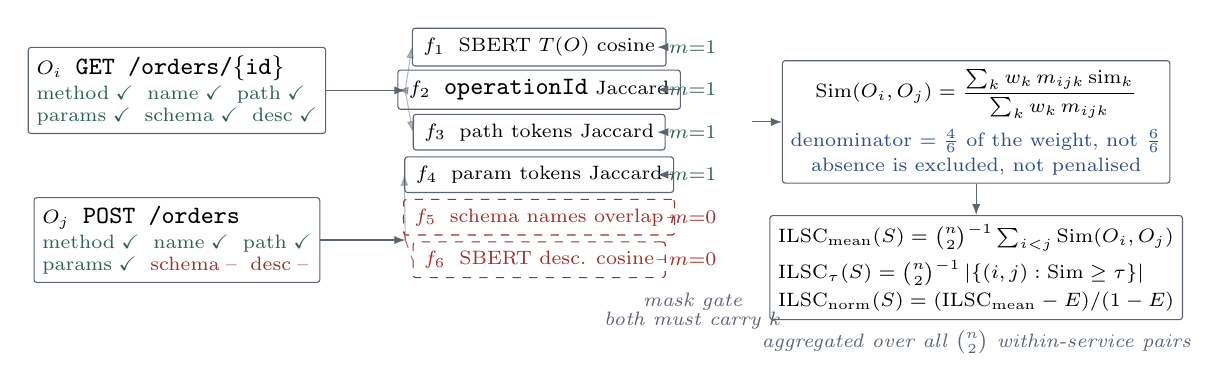
\begin{tikzpicture}[
  font=\scriptsize,
  box/.style={draw=inkgrey, rounded corners=1pt, align=left, inner sep=3pt},
  feat/.style={draw=inkgrey, rounded corners=1pt, minimum width=3.05cm,
               minimum height=0.44cm, align=left, inner xsep=4pt},
  featoff/.style={feat, draw=inkred, dashed, text=inkred},
  arr/.style={-{Latex[length=1.4mm]}, draw=inkgrey},
  arroff/.style={draw=inkred, dashed, opacity=0.7}
]

% ---- operations
\node[box, minimum width=2.9cm] (oi) at (0,0.95)
  {\textbf{$O_i$}\; \code{GET /orders/\{id\}}\\[1pt]
   \textcolor{inkgreen}{method\;$\checkmark$\; name\;$\checkmark$\; path\;$\checkmark$}\\
   \textcolor{inkgreen}{params\;$\checkmark$\; schema\;$\checkmark$\; desc\;$\checkmark$}};
\node[box, minimum width=2.9cm] (oj) at (0,-0.95)
  {\textbf{$O_j$}\; \code{POST /orders}\\[1pt]
   \textcolor{inkgreen}{method\;$\checkmark$\; name\;$\checkmark$\; path\;$\checkmark$}\\
   \textcolor{inkgreen}{params\;$\checkmark$}\;
   \textcolor{inkred}{schema\;--\; desc\;--}};

% ---- features
\node[feat] (f1) at (4.6, 1.50) {$f_1$\; SBERT $T(O)$ \hfill cosine};
\node[feat] (f2) at (4.6, 0.96) {$f_2$\; \code{operationId} \hfill Jaccard};
\node[feat] (f3) at (4.6, 0.42) {$f_3$\; path tokens \hfill Jaccard};
\node[feat] (f4) at (4.6,-0.12) {$f_4$\; param tokens \hfill Jaccard};
\node[featoff] (f5) at (4.6,-0.66) {$f_5$\; schema names \hfill overlap};
\node[featoff] (f6) at (4.6,-1.20) {$f_6$\; SBERT desc. \hfill cosine};

\draw[arr] (oi.east) -- (2.7,0.95) -- (2.9,0.95);
\draw[arr] (oj.east) -- (2.7,-0.95) -- (2.9,-0.95);
\draw[arr, opacity=0.45] (2.9,0.95) -- (f1.west);
\draw[arr, opacity=0.45] (2.9,0.95) -- (f2.west);
\draw[arr, opacity=0.45] (2.9,0.95) -- (f3.west);
\draw[arr, opacity=0.45] (2.9,-0.95) -- (f4.west);
\draw[arroff] (2.9,-0.95) -- (f5.west);
\draw[arroff] (2.9,-0.95) -- (f6.west);

% ---- mask gates
\foreach \n/\y in {f1/1.50, f2/0.96, f3/0.42, f4/-0.12}{
  \node[text=inkgreen] at (6.55,\y) {$m{=}1$};
  \draw[arr] (\n.east) -- (6.1,\y);
}
\foreach \n/\y in {f5/-0.66, f6/-1.20}{
  \node[text=inkred] at (6.55,\y) {$m{=}0$};
  \draw[arroff] (\n.east) -- (6.1,\y);
}
\node[align=center, text=inkgrey] at (6.55,-1.85)
  {\itshape mask gate\\[-1pt]\itshape both must carry $k$};

% ---- aggregation
\node[box, minimum width=4.3cm, align=center] (agg) at (10.15,0.55)
 {$\displaystyle \mathrm{Sim}(O_i,O_j)=
   \frac{\sum_k w_k\, m_{ijk}\, \mathrm{sim}_k}{\sum_k w_k\, m_{ijk}}$\\[3pt]
  \textcolor{inkblue}{denominator $=\tfrac{4}{6}$ of the weight, not $\tfrac{6}{6}$}\\[1pt]
  \textcolor{inkblue}{absence is excluded, not penalised}};
\draw[arr] (7.3,0.55) -- (agg.west);

\node[box, minimum width=4.3cm, align=left] (out) at (10.15,-1.30)
 {$\ilscm(S)=\binom{n}{2}^{-1}\sum_{i<j}\mathrm{Sim}(O_i,O_j)$\\[2pt]
  $\ilsct(S)=\binom{n}{2}^{-1}\,|\{(i,j):\mathrm{Sim}\ge\tau\}|$\\[2pt]
  $\ilscn(S)=(\ilscm-E)/(1-E)$};
\draw[arr] (agg.south) -- (out.north);

\node[text=inkgrey, align=left] at (10.15,-2.25)
 {\itshape aggregated over all $\binom{n}{2}$ within-service pairs};

\end{tikzpicture}
\caption{The \ilsc{} pipeline, drawn at the mask. Operation $O_j$ declares no
schema and no description, so $f_5$ and $f_6$ are gated off \emph{for this pair}
and disappear from both the numerator and the denominator: the four surviving
features share the whole weight rather than four sixths of it. A metric without
the mask would score the two missing features as $0$ and report the pair as
dissimilar on evidence that does not exist.}
\label{fig:arch}
\end{figure*}

\subsection{Aggregation and normalisation}
\begin{align}
\ilscm(S) &= \frac{2}{n(n-1)} \sum_{i<j} \mathrm{Sim}(O_i,O_j) \label{eq:mean}\\
\ilsct(S) &= \frac{|\{(i,j) : \mathrm{Sim}(O_i,O_j) \ge \tau\}|}{n(n-1)/2}
              \label{eq:tau}\\
\ilscn(S) &= \frac{\ilscm(S) - E[\mathrm{ILSC_{rand}}]}
                  {1 - E[\mathrm{ILSC_{rand}}]} \label{eq:norm}
\end{align}
with $\tau=0.50$ by default. $\ilscn$ is reported unclipped: a negative value
would mean the service is less coherent than an arbitrary bag of operations,
which is informative rather than an error.

\subsection{Null models}
Two null models are estimated by Monte Carlo over $400{,}000$ random pairs each.
The \emph{global} null draws operations from the whole corpus and answers ``is
this service more coherent than an arbitrary bag of API operations?''---a weak
bar, $E=0.0988$ (SE $0.00009$). The \emph{provider-restricted} null draws from
services sharing a publisher: median $0.2193$ over the $97$ providers with an
estimable pool, range $0.0917$--$0.5065$, with $96$ of $97$ above the global
figure. The gap between the two normalisations is itself a finding: a service
must clear a much higher bar to look coherent relative to its own publisher than
relative to the corpus at large. Pairs drawn from the same service are resampled,
since leaving them in would import exactly the within-service coherence the null
exists to be free of.

We originally specified a \emph{domain}-restricted null. No domain label source
survived: keyword labelling was rejected at $52\%$ agreement against a blind
human sample of $50$ services, and LLM labelling was rejected as circular with
the metric under test and impossible to pin for replication. Provider is
metadata, needs no annotator, and is a \emph{conservative} substitution, being
coarser than a domain.

\subsection{$E[\mathrm{ILSC_{rand}}]$ does not depend on $n$}
\label{sec:flat-null}
$\ilscm$ is a mean over exchangeable pairs, so its expectation equals that of a
single random pair for every $n$. We verify this at seven sizes with $1{,}000$
full draws each: $E$ ranges $0.0996$--$0.1016$ for $n=3\ldots200$, a spread of
$0.00203$. The consequence constrains what may be claimed: \emph{$\ilscn$ is an
affine rescaling of $\ilscm$ with constant coefficients.} It cannot reorder
services, every rank-based result is identical on either, and---as
Section~\ref{sec:res-size} shows---it cannot remove the metric's dependence on
service size. $\ilscn$ is worth reporting for interpretability and must not be
presented as independent evidence.

\subsection{Complexity}
Feature extraction is $O(|S|)$ in operations. Embedding is one forward pass per
unique text; our corpus of $97{,}912$ operations required $89{,}852$ unique
$T$ vectors and $54{,}701$ unique description vectors, cached once. Scoring is
$O(n^2)$ per service in pairs, blocked so that per-feature similarities are
computed once and reused. The full corpus scores in $51$~s on commodity
hardware after embedding.

% =============================================================================
\section{Study Design}
\label{sec:design}

\subsection{Research questions and hypotheses}
Table~\ref{tab:rqs} maps questions and hypotheses to experiments. Gate criteria
were fixed before any score existed: Gate~1 required the five hand-labelled
cohesive services to score clearly above the five mixed ones; Gate~2 required
pair-level $\rho \ge 0.4$, with $0.4$--$0.6$ to be reframed as ``moderate
correlation, complementary signal''.

\begin{table}[!t]
\caption{Research questions, hypotheses and the experiments that answer them.}
\label{tab:rqs}
\centering
\footnotesize
\begin{tabular}{@{}p{0.44cm}p{5.0cm}p{1.05cm}p{0.75cm}@{}}
\toprule
\textbf{ID} & \textbf{Question / hypothesis} & \textbf{Answered by} & \textbf{\S} \\
\midrule
RQ1 & How to define a static, theoretically grounded semantic cohesion metric on interfaces alone? & Model, Exp.~1 & \ref{sec:model} \\
RQ2 & How to compute pairwise similarity when spec fields are missing or auto-generated? & Mask, availability study & \ref{sec:res-avail} \\
RQ3 & Does interface similarity reflect code-level relatedness, per pair and per service? & Exp.~3 & \ref{sec:res-code} \\
RQ4 & Is \ilsc{} sensitive to semantic contamination specifically, rather than to size? & Exp.~2, Exp.~6 & \ref{sec:res-pert}, \ref{sec:res-size} \\
RQ5 & Is the ranking stable across weights and $\tau$? & Exp.~5 & \ref{sec:res-sens} \\
\midrule
H1 & Interface similarity correlates with code-based structural relatedness at the operation-pair level. & Exp.~3 & \ref{sec:res-code} \\
H2 & \ilsc{} degrades more under foreign-domain injection than under same-domain injection of equal size. & Exp.~2 & \ref{sec:res-pert} \\
H3 & Rankings are stable under reasonable variation of weights and $\tau$. & Exp.~5 & \ref{sec:res-sens} \\
\bottomrule
\end{tabular}
\end{table}

\subsection{Corpus}
\label{sec:design-corpus}
A single self-collected crawl invites the standard objection of dataset bias.
The corpus is therefore built from a source already used in peer-reviewed
work plus a current snapshot for recency, both pinned to a commit
(Table~\ref{tab:sources}). Every service carries a provenance column.

\begin{table}[!t]
\caption{Corpus sources, both pinned to a commit.}
\label{tab:sources}
\centering
\footnotesize
\begin{tabular}{@{}llr@{}}
\toprule
\textbf{ID} & \textbf{Source} & \textbf{Files} \\
\midrule
S1 & RAMA threshold benchmark~\cite{bogner2020rama} & $2{,}619$ \\
S2 & APIs.guru \code{openapi-directory} & $4{,}138$ \\
\midrule
   & \textbf{Total input} & $\mathbf{6{,}757}$ \\
\bottomrule
\end{tabular}
\end{table}

S1 is reused for \emph{comparability, not diversity}---a distinction worth
making, because S1 is the \emph{more} publisher-concentrated of the two sources
(Table~\ref{tab:concentration}). Reusing a published corpus buys comparability
with Bogner~et~al., not representativeness.

Curation proceeds in six logged stages (Fig.~\ref{fig:pipeline},
Table~\ref{tab:funnel}). Swagger~2.0 is converted rather than discarded:
dropping it would bias the sample toward recently published APIs and would have
eliminated the entire code-correlation benchmark, every specification of which
is 2.0. All $144$ conversions succeeded, and all $2{,}206$ surviving services
were verified to have an identical (method, path) operation set before and after
conversion---a mismatch is treated as a hard failure, since it would silently
move every downstream pairwise count.

% ------------------------------------------------------------ PIPELINE FIGURE
\begin{figure*}[!t]
\centering
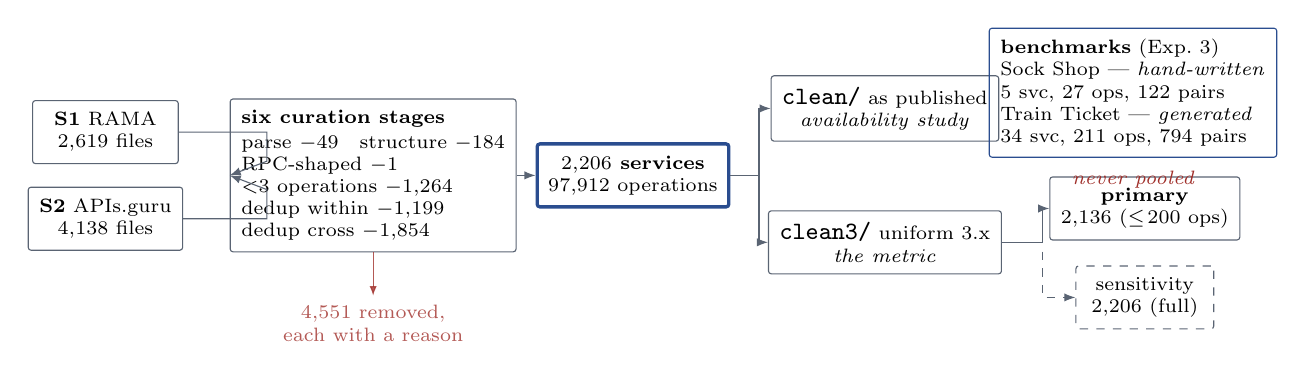
\begin{tikzpicture}[
  font=\scriptsize,
  b/.style={draw=inkgrey, rounded corners=1pt, align=center, inner sep=4pt,
            minimum height=0.8cm},
  strong/.style={b, very thick, draw=inkblue},
  arr/.style={-{Latex[length=1.4mm]}, draw=inkgrey},
  drop/.style={-{Latex[length=1.2mm]}, draw=inkred, opacity=0.8}
]
\node[b, minimum width=1.85cm] (s1) at (0,0.55) {\textbf{S1} RAMA\\$2{,}619$ files};
\node[b, minimum width=1.85cm] (s2) at (0,-0.55) {\textbf{S2} APIs.guru\\$4{,}138$ files};

\node[b, minimum width=2.55cm, align=left] (filt) at (3.4,0)
  {\textbf{six curation stages}\\[1pt]
   parse $-49$ \; structure $-184$\\
   RPC-shaped $-1$\\
   ${<}3$ operations $-1{,}264$\\
   dedup within $-1{,}199$\\
   dedup cross $-1{,}854$};
\draw[arr] (s1.east) -- (2.05,0.55) -- (2.05,0.18) -- (filt.west);
\draw[arr] (s2.east) -- (2.05,-0.55) -- (2.05,-0.18) -- (filt.west);
\draw[drop] (filt.south) -- ++(0,-0.55)
  node[below, text=inkred, align=center] {$4{,}551$ removed,\\each with a reason};

\node[strong, minimum width=1.9cm] (surv) at (6.7,0)
  {\textbf{$2{,}206$ services}\\$97{,}912$ operations};
\draw[arr] (filt.east) -- (surv.west);

\node[b, minimum width=2.35cm] (clean) at (9.9,0.85)
  {\code{clean/} as published\\\emph{availability study}};
\node[b, minimum width=2.35cm] (clean3) at (9.9,-0.85)
  {\code{clean3/} uniform 3.x\\\emph{the metric}};
\draw[arr] (surv.east) -- (8.3,0) -- (8.3,0.85) -- (clean.west);
\draw[arr] (surv.east) -- (8.3,0) -- (8.3,-0.85) -- (clean3.west);

\node[b, minimum width=1.75cm] (prim) at (13.2,-0.42)
  {\textbf{primary}\\$2{,}136$ ($\le\!200$ ops)};
\node[b, minimum width=1.75cm, dashed] (sens) at (13.2,-1.55)
  {sensitivity\\$2{,}206$ (full)};
\draw[arr] (clean3.east) -- (11.9,-0.85) -- (11.9,-0.42) -- (prim.west);
\draw[arr, dashed] (clean3.east) -- (11.9,-0.85) -- (11.9,-1.55) -- (sens.west);

\node[b, minimum width=2.6cm, align=left, draw=inkblue] (bench) at (13.05,1.05)
  {\textbf{benchmarks} (Exp.~3)\\
   Sock Shop --- \emph{hand-written}\\ 5 svc, 27 ops, 122 pairs\\
   Train Ticket --- \emph{generated}\\ 34 svc, 211 ops, 794 pairs};
\node[text=inkred, align=center] at (13.05,-0.05) {\itshape never pooled};

\end{tikzpicture}
\caption{Corpus collection and preprocessing. Two pinned sources enter six
logged curation stages; $2{,}206$ services survive and fork into an
as-published corpus, which the availability study measures, and a uniform
OpenAPI~3.x corpus, which the metric consumes. Specifications above $200$
operations describe API gateways rather than single-capability services and are
held out of the primary population, with every analysis repeated on the full
corpus as a sensitivity check. The two benchmark systems form a separate track
and are never pooled, because their specifications differ in provenance.}
\label{fig:pipeline}
\end{figure*}

\begin{table}[!t]
\caption{Curation funnel. Every removal is logged with its reason.}
\label{tab:funnel}
\centering
\footnotesize
\begin{tabular}{@{}llr@{}}
\toprule
\textbf{Stage} & \textbf{Reason} & \textbf{Removed} \\
\midrule
a & malformed file & $49$ \\
a & no \code{paths} or no \code{info} & $184$ \\
b & RPC-shaped (every path identical) & $1$ \\
c & fewer than $3$ operations & $1{,}264$ \\
d & duplicate within source (older version) & $1{,}199$ \\
e & duplicate across sources (present in S1) & $1{,}854$ \\
\midrule
  & \textbf{Total removed} & $\mathbf{4{,}551}$ \\
  & \textbf{Surviving services} & $\mathbf{2{,}206}$ \\
\bottomrule
\end{tabular}
\end{table}

\begin{table}[!t]
\caption{Corpus composition.}
\label{tab:composition}
\centering
\footnotesize
\begin{tabular}{@{}lr@{}}
\toprule
\textbf{Property} & \textbf{Value} \\
\midrule
Services (S1 / S2) & $2{,}206$ ($1{,}014$ / $1{,}192$) \\
Operations & $97{,}912$ \\
Operations per service (min / med / mean / max) & $3$ / $16$ / $44.4$ / $11{,}422$ \\
Within-service pairs (full / primary) & $77{,}611{,}030$ / $1{,}828{,}978$ \\
OpenAPI 3.x / Swagger 2.0 & $2{,}062$ / $144$ \\
Distinct providers & $616$ \\
Administrative endpoints stripped & $62$ (48 services) \\
Strict validation, seeded sample $n{=}200$ & $97.5\%$ valid \\
\bottomrule
\end{tabular}
\end{table}

\begin{table}[!t]
\caption{Publisher concentration, the study's main external-validity
constraint. The peer-reviewed source is the more concentrated one.}
\label{tab:concentration}
\centering
\footnotesize
\begin{tabular}{@{}lrrr@{}}
\toprule
& \textbf{Services} & \textbf{Providers} & \textbf{Top-3 cloud} \\
\midrule
S1 (RAMA) & $1{,}014$ & $315$ & $589$ ($58.1\%$) \\
S2 (APIs.guru) & $1{,}192$ & $460$ & $444$ ($37.4\%$) \\
Pooled & $2{,}206$ & $616$ & $1{,}033$ ($46.8\%$) \\
\bottomrule
\end{tabular}
\end{table}

\subsection{The oversized cap}
Above roughly $200$ operations a specification describes an API gateway or a
whole platform surface---one document in our corpus declares $11{,}422$
operations---rather than the single-capability microservice \ilsc{} is defined
over. Such specifications are flagged and held out of the \emph{primary}
population; every analysis is repeated on the full corpus as a
\emph{sensitivity} check, and both are reported. The justification is scope, not
compute: $200$ sits at the $96.8$th percentile of the size distribution.

The cap matters more than expected. The $70$ oversized services ($3.2\%$ of the
corpus) hold $97.6\%$ of all within-service pairs, and one service alone holds
$84.0\%$. Consequently every operation-weighted corpus statistic on the full
corpus is close to a statement about a handful of documents: pair-weighted
feature co-availability moves by up to $50$ points between the two populations,
while every per-service quartile boundary moves by at most $3.2$ points. This
asymmetry is the empirical case for reporting service-level rather than
pair-weighted statistics, and we do so throughout.

\subsection{Benchmark systems and the provenance split}
\label{sec:design-bench}
Experiment~3 correlates \ilsc{} against a code-level ground truth on two
benchmark systems (Table~\ref{tab:bench}). They are \emph{not} interchangeable.
Sock Shop's specifications are hand-written and independent of its source code.
Train Ticket~\cite{zhou2021fault} publishes no authored contract; the only
citable artifact derives its OpenAPI documents from the service code by
framework introspection. We therefore report $\rho_{\mathrm{independent}}$ and
$\rho_{\mathrm{derived}}$ \emph{separately and never pooled}, and treat the
distance between them as a measurable estimate of how much specification--code
derivation inflates the correlation.

A third system could not be added: Online Boutique is gRPC with no OpenAPI at
all, and its \code{.proto} methods are not (method, path) operations. The
hand-written condition therefore rests on one system, which we state as a
limitation rather than discover at review.

\begin{table}[!t]
\caption{Benchmark systems for Experiment~3. Corpus filters do not apply here:
these systems are selected, not sampled.}
\label{tab:bench}
\centering
\footnotesize
\begin{tabular}{@{}lccrrr@{}}
\toprule
\textbf{System} & \textbf{Origin} & \textbf{Svc} & \textbf{Ops} &
\textbf{Pairs} & \textbf{Role} \\
\midrule
Sock Shop & hand-written & $5$ & $27$ & $122$ & $\rho_{\mathrm{indep}}$ \\
Train Ticket & generated & $34$ & $211$ & $794$ & $\rho_{\mathrm{deriv}}$ \\
\midrule
\textbf{Total} & & $\mathbf{39}$ & $\mathbf{238}$ & $\mathbf{916}$ & --- \\
\bottomrule
\end{tabular}
\end{table}

\subsection{Code-level ground truth}
For each benchmark endpoint we extract the set of domain entity types the
implementation touches, tracing controller to service to repository to model
class, with an explicit exclusion list for framework and primitive types. Sock
Shop's $27$ endpoints were extracted by hand with a \code{file:line} reference on
every row; Train Ticket's $211$ were extracted automatically, joining $209$
($99.1\%$), with two services in other languages handled manually. The code-side
similarity of a pair is the Jaccard of its two entity sets.

Entity names are matched exactly, so \code{Assurance} and \code{AssuranceType}
score $0.00$ despite being plainly related. Every such case pushes a pair toward
``code says unrelated'' while the interface says related, biasing $\rho$
\emph{downward}. We record this rather than fix it: changing the ground truth
after seeing $\rho$ would have to be declared, and any change must apply
identically to both systems or the provenance comparison breaks.

\subsection{Statistical procedures}
Correlations are Spearman's $\rho$ throughout, because the code-side variable is
ordinal with heavy ties. Confidence intervals on benchmark correlations use a
\emph{cluster} bootstrap that resamples whole services rather than pairs: pairs
inside a service share operations and move together, and resampling pairs would
report a precision the design does not have. Group comparisons use Cliff's
$\delta$~\cite{cliff1993dominance} and exact one-sided sign or Wilcoxon tests.
Rank agreement across parameterisations uses Kendall's
$W$~\cite{kendall1939problem}. Regressions report cluster-robust standard errors
with the publisher as the cluster~\cite{cameron2011robust}. Where two AUCs are
computed on the same pairs we compare them by paired bootstrap rather than by
overlap of marginal intervals, since the latter is not a valid test for
correlated ROC curves~\cite{delong1988comparing}.

\subsection{Parameters}
All parameters are pinned (Table~\ref{tab:params}) and three of them are swept
rather than asserted (Section~\ref{sec:res-sens}).

\begin{table}[!t]
\caption{Pinned parameters. Three are swept in Experiment~5.}
\label{tab:params}
\centering
\footnotesize
\begin{tabular}{@{}llc@{}}
\toprule
\textbf{Parameter} & \textbf{Value} & \textbf{Swept} \\
\midrule
Feature weights & $1/6$ each, uniform & yes \\
$\tau$ & $0.50$ (grid $0.30$--$0.70$) & yes \\
Version-token dropping & enabled & yes \\
Embedding model & \code{all-MiniLM-L6-v2} & no \\
Infrastructural ratio & ${>}\,0.80$ of a service's ops & no \\
Oversized cap & $200$ operations & both reported \\
Minimum operations & $3$ & no \\
Null-model pair samples & $400{,}000$ & no \\
Bootstrap resamples & $2{,}000$ & no \\
Perturbation levels $\times$ draws & $\{0,1,2,3,5\} \times 10$ & no \\
Random seed & $42$ & --- \\
\bottomrule
\end{tabular}
\end{table}

% =============================================================================
\section{Results}
\label{sec:results}

\subsection{RQ2: specifications are incomplete, and it is a pair-level problem}
\label{sec:res-avail}
Per operation, a description is present on $73.0\%$ (micro) and $83.7\%$ (macro,
per-service mean); \code{operationId} on $88.4\%$/$85.4\%$; parameters on
$91.1\%$/$89.3\%$. Description and summary move in \emph{opposite} directions
between the two averages ($+10.7$ and $-11.4$ points), because a handful of very
large specifications under-document one and over-document the other---a
structural difference in how large specifications are written, not noise.

The mask, however, evaluates \emph{pairs}, and the pair-level picture is
different (Table~\ref{tab:coavail}). Co-availability is high for names and
parameters and low for schemas and descriptions. Most importantly, the
per-service distribution is strongly \emph{bimodal}: $31.6\%$ of services never
fire the mask at all and $32.3\%$ fire it on every pair
(Fig.~\ref{fig:maskfire}). The honest summary is therefore ``the mask materially
affects $68.4\%$ of services'', not an average.

\begin{table}[!t]
\caption{Pair-level feature co-availability and mask activity. Micro is
pair-weighted; macro is the per-service mean. The two diverge sharply because
$3.2\%$ of services hold $97.6\%$ of all pairs.}
\label{tab:coavail}
\centering
\footnotesize
\begin{tabular}{@{}lrrrr@{}}
\toprule
\textbf{Feature} & \textbf{micro} & \textbf{macro} & \textbf{S1} & \textbf{S2} \\
\midrule
$f_2$ name & $97.2$ & $83.0$ & $88.8$ & $97.5$ \\
$f_4$ parameters & $92.3$ & $84.7$ & $88.9$ & $92.5$ \\
$f_5$ schemas & $36.1$ & $74.0$ & $73.7$ & $34.7$ \\
$f_6$ description & $24.1$ & $81.5$ & $82.0$ & $22.0$ \\
\midrule
\textbf{Mask fires} & $90.6$ & $49.6$ & $44.2$ & $92.3$ \\
\midrule
\multicolumn{5}{@{}l}{\emph{Per-service distribution (primary population)}}\\
Services never firing the mask & \multicolumn{4}{r}{$31.6\%$} \\
Services always firing the mask & \multicolumn{4}{r}{$32.3\%$} \\
\textbf{Services materially affected} & \multicolumn{4}{r}{$\mathbf{68.4\%}$} \\
\bottomrule
\end{tabular}
\end{table}

\begin{figure}[!t]
\centering
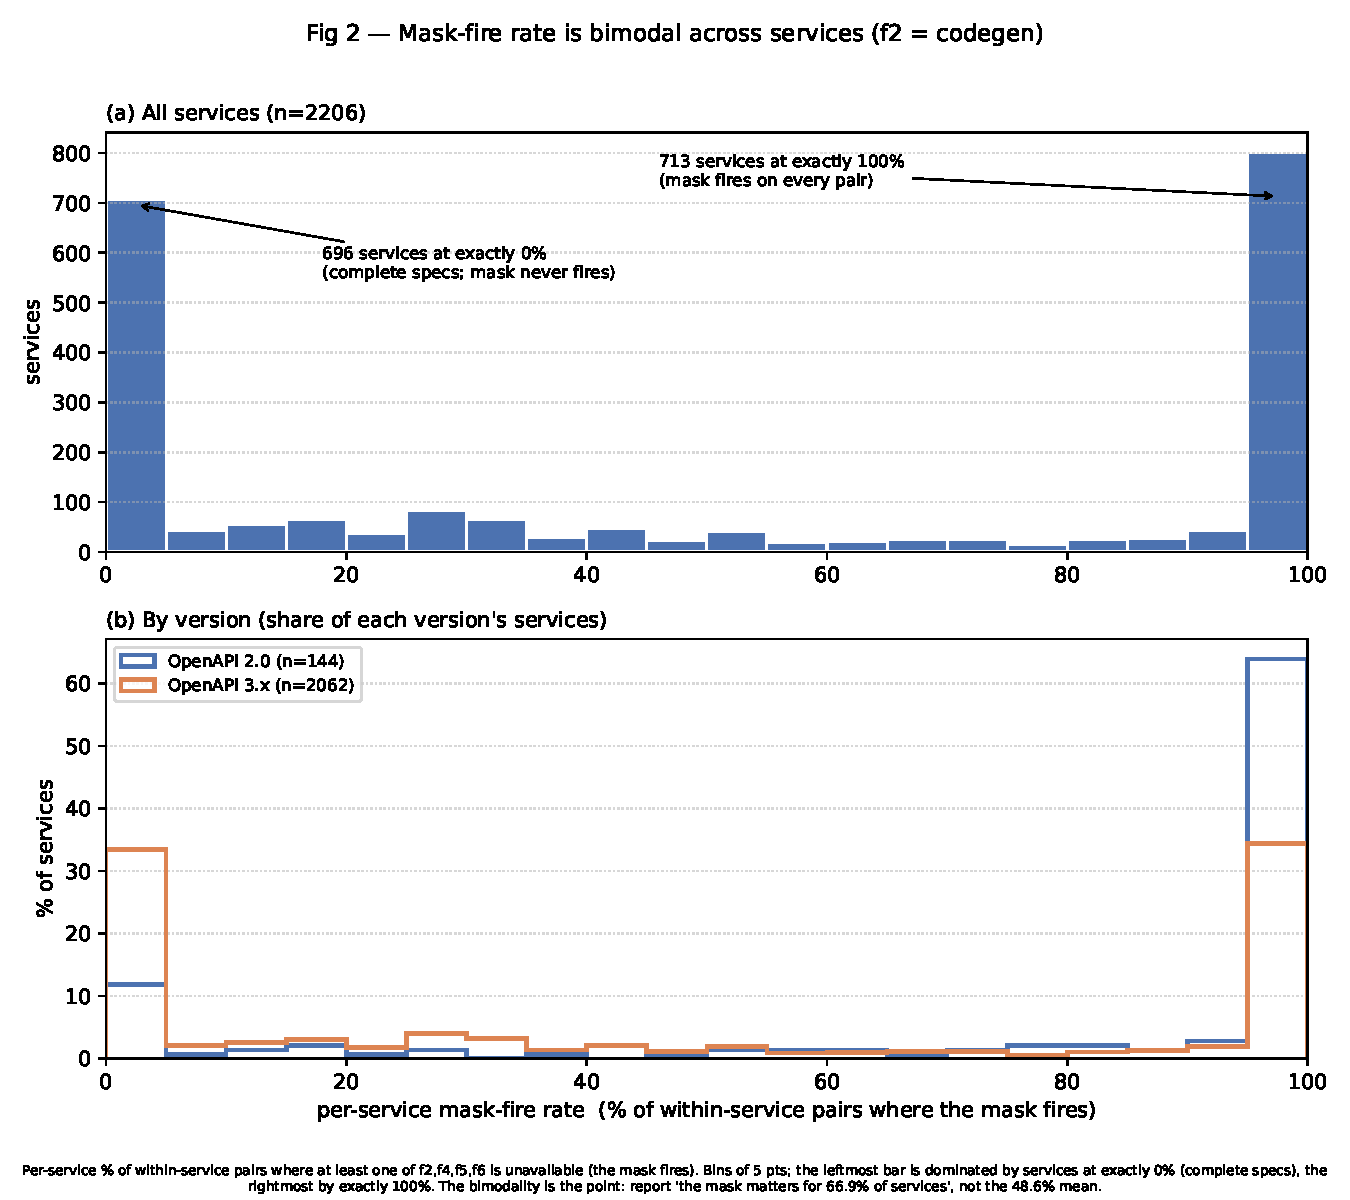
\includegraphics[width=\columnwidth]{fig2_maskfire_distribution.pdf}
\caption{Distribution of mask activity across services. The distribution is
bimodal---complete specifications the mask never changes, and specifications
where it fires on every pair---so a mean is the wrong summary and we report the
proportion of services materially affected.}
\label{fig:maskfire}
\end{figure}

Two robustness notes. The \code{operationId} ``informativeness'' definition
moves the pair-weighted headline by only $3.2$ points across three definitions,
though it moves the service-level figure by $13$ points, which we report as a
band rather than a point. And the availability study measures specifications as
published while the metric consumes converted ones; the two diverge on
parameters for the $144$ converted services ($96.4\%$ against $91.0\%$), making
the reported $f_4$ co-availability about five points optimistic for that subset.
A stated five-point discrepancy on one feature is a limitation; an unstated one
would be a defect.

\subsection{RQ1: distribution, thresholds, and feature non-redundancy}
\label{sec:res-thresholds}
Across the primary population of $2{,}136$ services, $\ilscm$ has mean $0.379$,
median $0.366$ and interquartile range $[0.285,0.453]$, spanning
$0.125$--$0.887$ with \emph{no} service saturating at either bound. The full
corpus differs by $0.003$ at the median, exactly as the size analysis predicts:
per-service statistics are robust to the oversized cap even though pair-weighted
ones are not.

Quartile thresholds are reported per population (Table~\ref{tab:thresholds});
the S1-only row is the one comparable with RAMA. S1 scores about $0.05$ above S2
at every quartile, so a quoted threshold must name the population that produced
it. Section~\ref{sec:res-size} adds the size stratification that we consider
mandatory for practical use.

\begin{table}[!t]
\caption{$\ilscm$ quartile thresholds by population. The S1-only row is the
RAMA-comparable one.}
\label{tab:thresholds}
\centering
\footnotesize
\begin{tabular}{@{}lrrrrr@{}}
\toprule
\textbf{Population} & \textbf{$n$} & \textbf{min} & \textbf{Q1} &
\textbf{median} & \textbf{Q3} \\
\midrule
Primary, all & $2{,}136$ & $0.125$ & $0.285$ & $0.366$ & $0.453$ \\
Primary, S1 only & $991$ & $0.141$ & $0.308$ & $0.388$ & $0.483$ \\
Primary, S2 only & $1{,}145$ & $0.125$ & $0.272$ & $0.346$ & $0.430$ \\
Sensitivity, all & $2{,}206$ & $0.125$ & $0.281$ & $0.363$ & $0.449$ \\
Sensitivity, S1 & $1{,}014$ & $0.141$ & $0.302$ & $0.385$ & $0.480$ \\
\bottomrule
\end{tabular}
\end{table}

The obvious objection to a six-feature metric is that the features measure the
same thing. Over $930{,}936$ sampled pairs, computed pairwise-complete so that a
masked feature is absent rather than zero, the maximum inter-feature Spearman
correlation is $0.558$ ($f_1$--$f_3$), well below the $0.85$ redundancy
threshold we set in advance (Fig.~\ref{fig:featcorr}). $f_1$ correlates most
with everything, which is expected since $T(O_i)$ is built from the same
material $f_2$--$f_5$ measure discretely, and $f_5$ is the most independent of
the lexical features ($\rho \le 0.24$), which justifies giving it a different
similarity function.

\begin{figure}[!t]
\centering
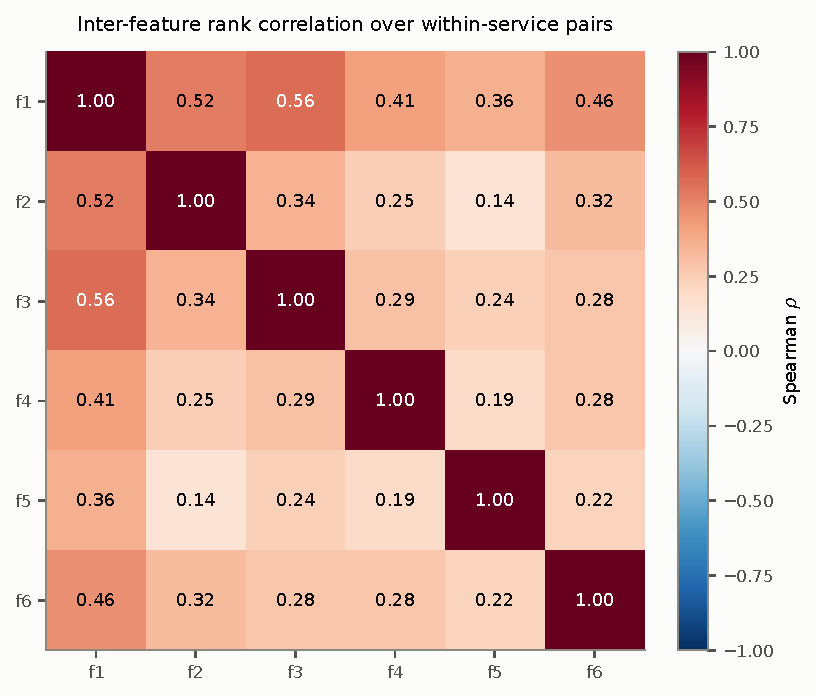
\includegraphics[width=0.86\columnwidth]{fig9_feature_correlation.pdf}
\caption{Inter-feature Spearman correlation over $930{,}936$ sampled
within-service pairs. No pair reaches $0.85$; the maximum is $0.558$.}
\label{fig:featcorr}
\end{figure}

An unplanned face-validity observation: the lowest-scoring service among all
$2{,}206$ is a general-purpose API whose own author declares six unrelated
domains (data tools, e-commerce, geolocation, imaging, security and networking,
telephony). That label was written before any score existed. The top of the
distribution is equally readable---small, single-purpose APIs.

\subsection{RQ4 / H2: perturbation against a size-matched control}
\label{sec:res-pert}
Injecting a foreign operation must lower a mean-similarity score by
construction, so the bare claim carries no evidential weight. We therefore run
three conditions at matched injection sizes and compare \emph{slopes}: injection
from the nearest sibling service of the same publisher, from any service of the
same publisher, and from a service of a different publisher. Twenty
top-quartile services, at most three per publisher, at levels
$\{0,1,2,3,5\}$ with ten draws each.

\begin{table}[!t]
\caption{Experiment~2. Degradation slope per injected operation, by semantic
distance. The three conditions order exactly as the proximity proxy predicts.}
\label{tab:perturbation}
\centering
\footnotesize
\begin{tabular}{@{}lrr@{}}
\toprule
\textbf{Condition} & \textbf{Slope} & \textbf{Monotonic} \\
\midrule
Same service (nearest sibling) & $-0.0350$ & --- \\
Same provider (control) & $-0.0654$ & --- \\
Cross provider (treatment) & $\mathbf{-0.0877}$ & $20/20$ \\
\midrule
Paired gap (treatment $-$ control) & $-0.0223$ & $20/20$ negative \\
Exact sign-flip $p$ & \multicolumn{2}{r}{$9.5\times10^{-7}$} \\
\bottomrule
\end{tabular}
\end{table}

All $20$ services degrade monotonically under the treatment, the three slopes
order exactly as semantic distance predicts, and the paired gap is negative for
every service (Table~\ref{tab:perturbation}, Fig.~\ref{fig:perturbation}).
\textbf{H2 is supported.} The ordering of all three conditions is a stronger
result than the two-condition contrast we designed for: it shows the
publisher-proximity proxy does not merely label, it graduates.

\begin{figure}[!t]
\centering
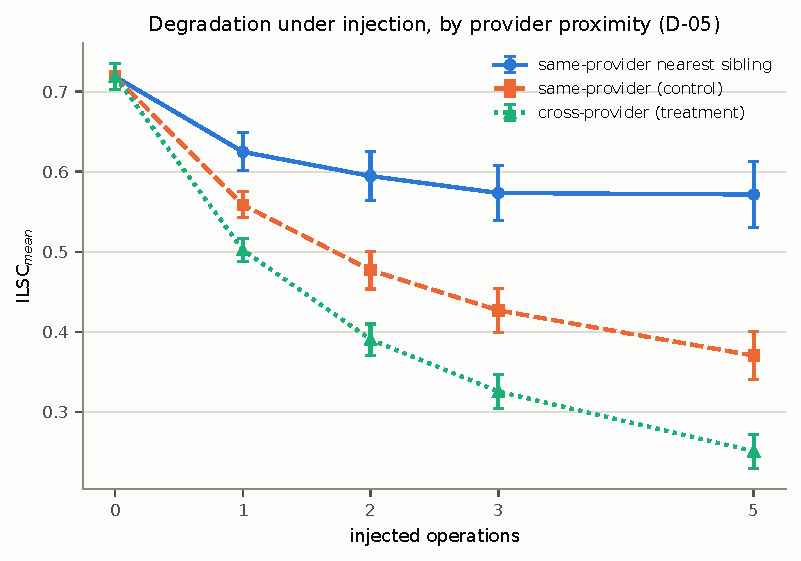
\includegraphics[width=\columnwidth]{fig3_perturbation.pdf}
\caption{Experiment~2. \ilsc{} under injection at five levels in three
conditions of increasing semantic distance. The evidential content is the
separation between the curves, not the fall of any one of them.}
\label{fig:perturbation}
\end{figure}

Two caveats. The $20$ targets are drawn from the top quartile, and because
\ilsc{} decreases with size (Section~\ref{sec:res-size}) they are small: a
median of $5$ operations against a corpus median of $16$. H2 is therefore
demonstrated on small services, and generalisation to larger ones is untested.
Second, the same-service control cannot supply five foreign operations for the
smallest targets, leaving $5$ of $80$ control cells empty; because degradation
curves flatten, this makes the control slope steeper than it would otherwise be
and the comparison correspondingly conservative.

\subsection{RQ3 / H1: correlation with code-level relatedness}
\label{sec:res-code}
Of $916$ within-service benchmark pairs, $906$ joined to a code row.
Table~\ref{tab:codecorr} reports both conditions.

\begin{table}[!t]
\caption{Experiment~3. Interface similarity against code-level entity overlap,
reported separately by specification provenance and never pooled.}
\label{tab:codecorr}
\centering
\footnotesize
\begin{tabular}{@{}lrr@{}}
\toprule
& \textbf{$\rho_{\mathrm{indep}}$} & \textbf{$\rho_{\mathrm{deriv}}$} \\
& Sock Shop & Train Ticket \\
& hand-written & generated \\
\midrule
Pairs / services & $122$ / $4$ & $790$ / $31$ \\
Services with code-side variance & $2$ & $29$ \\
Ground-truth levels (largest tie) & $5$ ($27.9\%$) & $16$ ($33.2\%$) \\
\midrule
\textbf{Spearman $\rho$ (pair level)} & $\mathbf{0.409}$ & $\mathbf{0.486}$ \\
$p$ & $3.0\times10^{-6}$ & $3.9\times10^{-48}$ \\
$95\%$ CI, pair bootstrap & $[0.243,0.547]$ & $[0.431,0.542]$ \\
$95\%$ CI, cluster bootstrap & $[0.318,0.643]$ & $[0.387,0.579]$ \\
$\rho$, service level & $0.738$ ($n{=}4$) & $0.513$ ($n{=}31$) \\
\midrule
\multicolumn{3}{@{}l}{Derivation inflation $= 0.486-0.409 = \mathbf{+0.078}$}\\
\bottomrule
\end{tabular}
\end{table}

Both coefficients land in the $0.4$--$0.6$ band that we specified in advance be
read as \emph{moderate correlation, complementary signal}: the interface and the
code carry partly independent information. We adopt that reading, and we do not
claim H1 as established. The cluster-bootstrap interval on the hand-written
condition straddles the $0.4$ threshold, and the reason is visible in the design
rather than the result: only two of four Sock Shop services have any code-side
variance at all, because the other two are genuinely single-aggregate services
in which every endpoint touches the same entity set. The condition the argument
would most like to lean on is the weaker-powered one, and the condition
quarantined for circularity is the better-powered one.

The derivation-inflation estimate of $+0.078$ is positive, as the two-condition
design predicted, but small---derivation inflates this correlation by roughly
eight points, not by enough to manufacture a finding.

$102$ of $906$ pairs ($11.3\%$) are discordant, and both anticipated kinds
appear. In one, a pair shares a path prefix and four of five path tokens but
touches disjoint entities (interface $0.86$, code $0.00$). In the other,
\code{GET /customers} and \code{POST /register} both touch the user entity
(code $1.00$) while sharing no lexical material at all
($f_2=f_3=f_5=0.00$)---scoring above zero \emph{only} through the embedding
feature. That pair is the study's clearest single piece of evidence that $f_1$ is
not redundant with the lexical features.

\subsection{Baselines and the ground-truth head-to-head}
\label{sec:res-4b}
Both baselines are implemented faithfully, which means without what \ilsc{}
adds: no availability mask, no infrastructural exclusion, no embeddings. They
read the same parsed corpus with the same administrative exclusions, so the
comparison differs in method, not in inputs.

On the corpus, \ilsc{} discriminates where the baselines saturate
(Table~\ref{tab:baselines}). LoCmsg's interquartile range is exactly zero: at
least half the corpus receives an identical score. \ilsc{} saturates on no
service at all.

\begin{table}[!t]
\caption{Corpus-level discrimination, primary population ($n{=}2{,}136$).
Saturation is the share of services receiving the maximum score, where the
metric can no longer distinguish anything.}
\label{tab:baselines}
\centering
\footnotesize
\begin{tabular}{@{}lrrrr@{}}
\toprule
\textbf{Metric} & \textbf{mean} & \textbf{IQR} & \textbf{distinct} &
\textbf{saturated} \\
\midrule
\ilsc{} & $0.379$ & $\mathbf{0.167}$ & $2{,}015$ & $\mathbf{0.0\%}$ \\
SIDC & $0.548$ & $0.862$ & $709$ & $35.8\%$ \\
$1-$LoCmsg & $0.916$ & $\mathbf{0.000}$ & $356$ & $76.9\%$ \\
\bottomrule
\end{tabular}
\end{table}

Under perturbation the picture is mixed and we report it as it fell
(Table~\ref{tab:baselinepert}). \ilsc{}'s foreign-versus-control gap exceeds
SIDC's, both raw and standardised, and \ilsc{} discriminates on $20$ of $20$
services against SIDC's $13$. Against LoCmsg the gap is \emph{larger} than
\ilsc{}'s and the superiority claim is \textbf{not} available. The context is
worth stating without using it as a rescue: LoCmsg scores exactly $0.000$ for
all $20$ test services \emph{before} any perturbation, so it cannot rank them at
all and can only fall once foreign operations arrive. A large degradation gap
measured from a saturated floor shows that a metric detects the arrival of
something foreign; it does not show that it measures how cohesive a service is.

\begin{table}[!t]
\caption{Experiment~4. Perturbation sensitivity of all three metrics on
identical injections. \ilsc{} beats SIDC and loses to LoCmsg, which is reported
rather than explained away.}
\label{tab:baselinepert}
\centering
\footnotesize
\begin{tabular}{@{}lrrrr@{}}
\toprule
\textbf{Metric} & \textbf{Gap} & \textbf{Gap in SD} &
\textbf{Neg.} & \textbf{$p$} \\
\midrule
\ilsc{} & $-0.0223$ & $-0.179$ & $20/20$ & $<10^{-6}$ \\
SIDC & $-0.0185$ & $-0.045$ & $13/20$ & $4.4\times10^{-3}$ \\
LoCmsg & $\mathbf{-0.0535}$ & $\mathbf{-0.256}$ & $19/20$ & $8.6\times10^{-6}$ \\
\bottomrule
\end{tabular}
\end{table}

The discrimination argument is itself contestable: \ilsc{} is a mean of six
continuous similarities while the baselines are proportions over pair counts, so
comparing their spreads shows \ilsc{} is more \emph{continuous}, not more
\emph{valid}. The test that settles it uses the external ground truth already
available. We decompose each baseline to the pair predicate its published
definition counts---SIDC to ``the two operations share at least one data type'',
LoCmsg to ``their message terms intersect''---and ask which predictor better
separates related from unrelated pairs. AUC is the primary figure because two of
the three predictors are binary and a correlation coefficient would penalise
them for their own coarseness.

\begin{table}[!t]
\caption{Experiment~4b. AUC against code-level relatedness. Provenance decides
the winner.}
\label{tab:auc}
\centering
\footnotesize
\begin{tabular}{@{}lrrr@{}}
\toprule
\textbf{Condition} & \textbf{\ilsc{}} & \textbf{SIDC} & \textbf{LoCmsg} \\
\midrule
Independent (hand-written) & $\mathbf{0.794}$ & $0.574$ & $0.651$ \\
Derived (generated) & $0.739$ & $0.917$ & $\mathbf{0.953}$ \\
\midrule
\multicolumn{4}{@{}l}{\emph{Paired bootstrap, independent condition}}\\
$\ilsc{} - $ SIDC & \multicolumn{3}{r}{$+0.179$ \; $[+0.069,+0.284]$} \\
$\ilsc{} - $ LoCmsg & \multicolumn{3}{r}{$+0.136$ \; $[+0.041,+0.226]$} \\
\bottomrule
\end{tabular}
\end{table}

On hand-written specifications \ilsc{} wins, and the paired differences exclude
zero (Table~\ref{tab:auc}, Fig.~\ref{fig:auc}). On generated specifications it
loses badly, and the reason is measurable: $29$ of $36$ schema names in the
generated contract ($81\%$) are also code entity names, against $3$ of $20$
($15\%$) in the hand-written one. In a generated specification the schema
vocabulary largely \emph{is} the code's type vocabulary---the generator
transliterates implementation types into the contract---so a metric that matches
schema names is reading the code's identifiers through a thin wrapper, and its
accuracy against a code-derived ground truth is near-tautological.

This sharpens the provenance finding considerably. Derivation does not merely
inflate a coefficient by $0.078$; it \emph{inverts which metric appears best}.
Because several widely used microservice benchmarks ship code-derived contracts,
any interface-metric evaluation conducted on them will favour the most
superficial metric as an artifact of provenance.

\begin{figure}[!t]
\centering
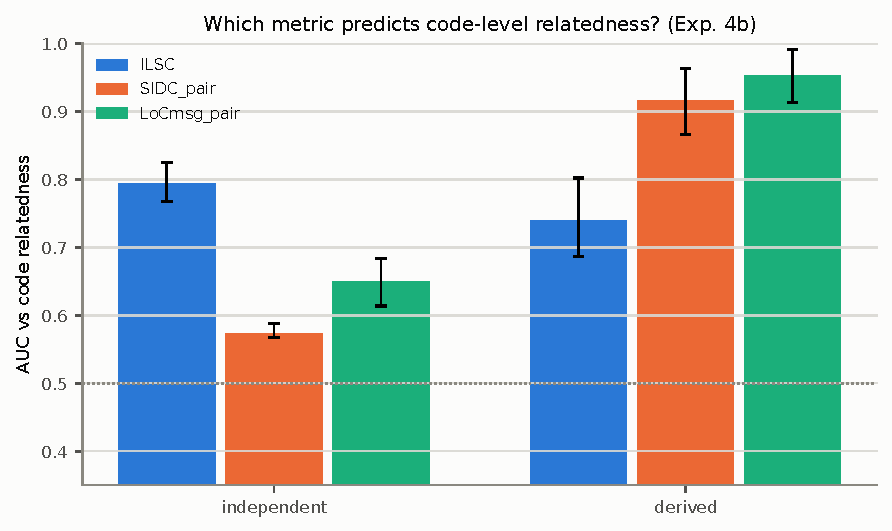
\includegraphics[width=\columnwidth]{fig8_baseline_auc.pdf}
\caption{Experiment~4b. Prediction of code-level relatedness by specification
provenance. The ranking of the three metrics reverses between hand-written and
generated contracts.}
\label{fig:auc}
\end{figure}

We state the limits of the winning condition plainly: it rests on $122$ pairs
over four services, of which only one contributes unrelated pairs, so the
interval is wide and the claim is about one system's hand-written contracts
rather than about hand-written contracts as a class.

\subsection{RQ5 / H3: sensitivity to weights, threshold and tokenisation}
\label{sec:res-sens}
Across $29$ weight configurations over $2{,}136$ services, Kendall's
$W = 0.9949$ on the $\pm20/40\%$ family---the H3 test---and $0.9671$ including
deliberately extreme schemes. The worst single $\pm40\%$ perturbation still
ranks at $\rho = 0.990$ against the pinned baseline. \textbf{H3 holds.} The
equal weighting is defensible because the choice barely matters, not because it
was tuned; no weighting was changed at any point in the study.

One configuration deserves its own sentence rather than burial: switching five
of six features off entirely (\code{f1\_only}) still reaches $\rho = 0.808$
against the full metric. The honest framing is that \emph{$f_1$ carries the
largest share of the ranking signal and the remaining five refine it}, not that
six features contribute equally. Fig.~\ref{fig:featcorr} keeps this from
collapsing further: no feature pair correlates above $0.558$, so the other five
are not redundant with $f_1$, they are smaller contributors.

Sweeping $\tau$ from $0.30$ to $0.70$ moves both edge density
($0.590 \rightarrow 0.083$) and mean component count
($1.58 \rightarrow 15.38$) smoothly, with no discontinuity that would make a
nearby threshold qualitatively different (Fig.~\ref{fig:tau}). $\tau=0.50$ sits
mid-range on both curves, which is the argument for it---not that it optimises
anything, but that it is where the statistic still varies.

\begin{figure}[!t]
\centering
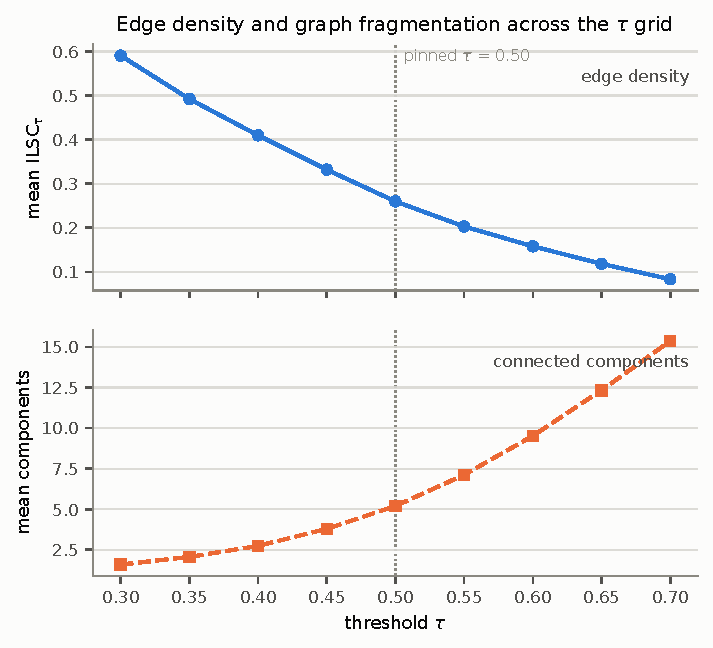
\includegraphics[width=\columnwidth]{fig6_tau_sweep.pdf}
\caption{The $\tau$ sweep. Both curves are smooth across the usable range;
$\tau = 0.50$ is a position, not an optimum.}
\label{fig:tau}
\end{figure}

A third knob cannot be swept by reweighting, because it changes the tokenizer
and therefore the embeddings: whether version tokens are dropped. Re-parsing and
re-embedding the whole corpus with the flag disabled changes the ranking
negligibly ($\rho = 0.998$, Kendall $\tau = 0.989$) but moves the $74$ services
it actually touches by $+0.027$ on average and one service by $+0.121$. The
direction confirms why the setting exists: disabling it makes every versioned
path share a spurious token. Experiment~5 is therefore a three-knob sensitivity
analysis.

\subsection{Size dependence, and construct validity under size control}
\label{sec:res-size}
The finding that constrains practical use of \ilsc{} is one we did not
anticipate. Over the primary population, $\ilscm$ correlates with operation
count at Spearman $\rho = -0.5505$ ($p = 1.7\times10^{-169}$), and the
relationship is monotonic across every size band (Table~\ref{tab:sizebands},
Fig.~\ref{fig:sizetags}).

The null-model normalisation cannot correct this. Section~\ref{sec:flat-null}
establishes that $E[\mathrm{ILSC_{rand}}(n)]$ is flat in $n$; it follows
immediately that $\ilscn$ is an affine rescale of $\ilscm$ and inherits the
dependence in full, which we confirm---$\ilscn$ correlates with operation count
at exactly the same $-0.5505$. We therefore withdraw any claim that the
null-model normalisation is a \emph{size} normalisation. It answers ``how far
above chance is this service'', which is a different and still useful question.

\begin{table}[!t]
\caption{$\ilscm$ quartile thresholds stratified by service size, primary
population. A single pooled threshold grades a service largely on how many
operations it declares; these are the thresholds we recommend for practical
use.}
\label{tab:sizebands}
\centering
\footnotesize
\begin{tabular}{@{}lrrrrr@{}}
\toprule
\textbf{Band (ops)} & \textbf{$n$} & \textbf{Q1} & \textbf{median} &
\textbf{Q3} & \textbf{S1 median} \\
\midrule
$3$--$5$ & $380$ & $0.369$ & $0.470$ & $0.572$ & $0.495$ \\
$6$--$10$ & $430$ & $0.350$ & $0.430$ & $0.515$ & $0.465$ \\
$11$--$20$ & $485$ & $0.306$ & $0.381$ & $0.443$ & $0.404$ \\
$21$--$50$ & $528$ & $0.267$ & $0.327$ & $0.377$ & $0.360$ \\
$51$--$200$ & $313$ & $0.219$ & $0.266$ & $0.328$ & $0.284$ \\
\midrule
Pooled & $2{,}136$ & $0.285$ & $0.366$ & $0.453$ & $0.388$ \\
\bottomrule
\end{tabular}
\end{table}

\begin{figure}[!t]
\centering
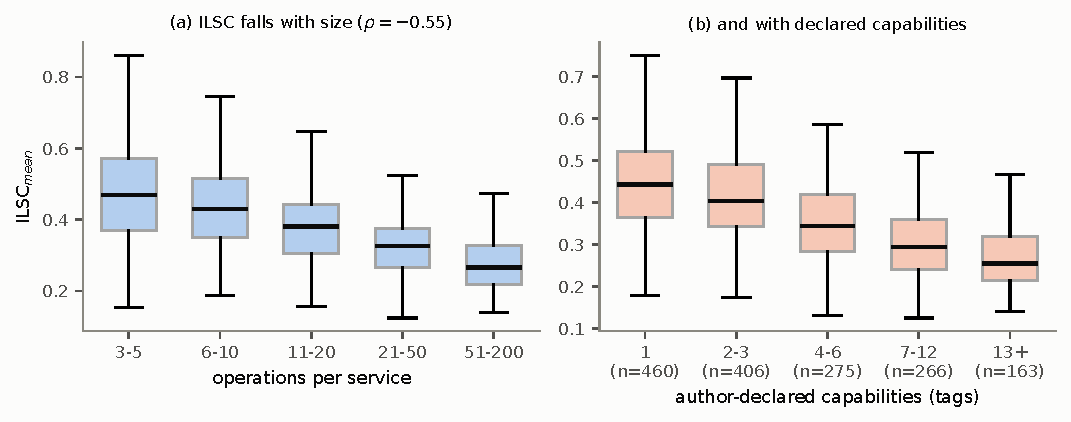
\includegraphics[width=\columnwidth]{fig11_size_and_tags.pdf}
\caption{\ilsc{} falls both with service size (a) and with the number of
capabilities the author declares (b). The two are themselves correlated at
$\rho = 0.667$, which is why separating them requires a corpus-scale regression
rather than a matched design.}
\label{fig:sizetags}
\end{figure}

This raises the construct question directly: does \ilsc{} respond to how many
\emph{capabilities} a service declares, or only to how \emph{large} it is? We
first attempted a matched design---for every publisher offering both a
single-capability and a many-capability service, compare one of each within the
publisher, using the author's own OpenAPI tag count as a label independent of
every \ilsc{} feature. Across $16$ publishers the single-capability service
scored higher in $14$ cases, mean difference $+0.105$, Wilcoxon
$p = 0.00056$.

That design does not settle the question, and we report why rather than
present it as if it did. The single-capability side is a median of $9$
operations against $52$---smaller in $15$ of $16$ pairs. Drawing random services
from the corpus at exactly those two sizes and ignoring capability entirely
reproduces the effect (size-only null $+0.091$, $95\%$ interval
$[+0.027,+0.155]$; $P(\text{null} \ge \text{observed}) = 0.335$). At $16$ pairs
the design cannot separate two variables that are themselves correlated at
$\rho = 0.667$.

The corpus can. We regress $\ilscm$ on both terms over the $1{,}570$ services
that carry at least one author tag, with publisher fixed effects and standard
errors clustered by publisher (Table~\ref{tab:regression}). Each term
alone explains a similar amount; entered together, \emph{both survive}. With
publisher held fixed as well, a doubling of the declared capability count is
associated with a $0.017$ decrease in $\ilscm$
($p = 0.006$), and a doubling of size with a $0.030$ decrease
($p < 10^{-10}$). The distribution-free companion agrees: the partial Spearman
correlation between \ilsc{} and capability count, controlling for operation
count, is $-0.279$ ($p = 2.3\times10^{-29}$).

\begin{table}[!t]
\caption{Construct validity under size control. OLS on $1{,}570$ services with
at least one author-declared tag; cluster-robust standard errors, $503$
publisher clusters. The capability term survives the size term and publisher
fixed effects.}
\label{tab:regression}
\centering
\footnotesize
\begin{tabular}{@{}llrrr@{}}
\toprule
\textbf{Model} & \textbf{Term} & \textbf{$\beta$} & \textbf{SE} &
\textbf{$p$} \\
\midrule
M1 & $\log_2(\text{tags})$ & $-0.0473$ & $0.0065$ & $4.8\times10^{-13}$ \\
M2 & $\log_2(\text{ops})$ & $-0.0479$ & $0.0046$ & $<10^{-15}$ \\
\midrule
\multirow{2}{*}{M3} & $\log_2(\text{tags})$ & $-0.0250$ & $0.0064$ & $1.0\times10^{-4}$ \\
 & $\log_2(\text{ops})$ & $-0.0311$ & $0.0059$ & $1.4\times10^{-7}$ \\
\midrule
\multirow{2}{*}{M4$^{\dag}$} & $\log_2(\text{tags})$ & $\mathbf{-0.0172}$ & $0.0062$ & $\mathbf{0.0056}$ \\
 & $\log_2(\text{ops})$ & $-0.0297$ & $0.0045$ & $4.7\times10^{-11}$ \\
\midrule
\multicolumn{2}{@{}l}{Partial Spearman (tags $\mid$ ops)} & $-0.279$ & --- & $2.3\times10^{-29}$ \\
\bottomrule
\multicolumn{5}{@{}l}{\footnotesize $^{\dag}$ adds fixed effects for the $23$ publishers with ${\ge}5$ services; $R^2 = 0.55$.}
\end{tabular}
\end{table}

The construct claim therefore holds, but in a weaker and more precise form than
the matched design suggested: \ilsc{} responds to the number of capabilities a
service declares \emph{and} to its size, with the size effect the larger of the
two. Both are real, and a user of the metric needs to know both. This is why we
publish thresholds per size band: applied naively, a pooled threshold would let
a practitioner move a service from red to green by splitting its specification
in half.

\subsection{What the metric's own validation revealed}
\label{sec:res-gate}
Our original ten-service sanity check---five services hand-labelled cohesive and
five mixed, with written justifications recorded before any score
existed---\textbf{failed} (Cliff's $\delta = +0.200$, $p = 0.36$, no clean
separation). We report the failure and its diagnosis, because the diagnosis is
more informative than a pass would have been.

The check read as marginal ($\delta = +0.680$) \emph{before} we applied the
infrastructural-parameter exclusion to $f_4$. That exclusion moved the cohesive
candidates and left four of five mixed ones untouched, because the mixed ones
had no boilerplate to remove. Three of the five cohesive candidates were
hyperscaler services and none of the mixed ones was---and hyperscalers publish
narrowly scoped single-capability contracts as house style, which is exactly
the criterion the cohesive label used. A meaningful part of the earlier
separation was \ilsc{} separating publishers rather than cohesion. The failure
of a gate is what surfaced a genuine defect in the metric, which is the argument
for pre-registering such checks and reporting them when they fail.

One candidate is a construct finding rather than a measurement error. A payroll
service, hand-labelled cohesive, scores lowest of the cohesive group. Its tokens
are correct: it covers roughly ten distinct payroll resources within one business
capability, and the lexical overlap between employees and superannuation funds
is genuinely zero. No weighting rescues it, and Experiment~5 explains why---no
reasonable reweighting moves any ranking at all. We conclude that \ilsc{}
measures \emph{resource-level} cohesion, not \emph{capability-level} cohesion,
and that this belongs in the metric's definition rather than only in a threats
section.

% =============================================================================
\section{Discussion}
\label{sec:discussion}

\subsection{Resource-level versus capability-level cohesion}
The sharpest lesson from validation is a scope limit the design did not
anticipate. A service can serve exactly one business capability through many
lexically and structurally unrelated resources, and \ilsc{} will score it low.
That is correct by the metric's own definition and misleading if a reader
expects the other notion. Practitioners should read a low \ilsc{} as ``this
contract's operations do not resemble one another'', which is a prompt to
examine the service, not a verdict that it is badly designed.

\subsection{Specification provenance is a methodological hazard}
Experiment~4b's inversion is, we believe, the most transferable result here.
Interface-level metrics are routinely evaluated on benchmark systems, and
several widely used microservice benchmarks ship contracts generated from their
own source code. On such systems a metric that matches schema names against code
entity names is measuring the generator's transliteration, and will beat a
semantic metric by a wide margin. Any future evaluation of interface metrics
against code-derived ground truth should report specification provenance as a
first-class experimental variable, and should not pool systems that differ in
it.

\subsection{Size, thresholds, and how not to use them}
The size dependence is not a defect to be normalised away, but it is a hazard for
the practical artifact. Cohesion measured as mean pairwise similarity has an
arithmetic tendency to fall with $n$: more operations means more opportunities
for a dissimilar pair, and the mean is over all of them. Our regression shows
this is not \emph{only} arithmetic---declared capability count predicts \ilsc{}
independently---but the size term is the larger one. We therefore publish
size-stratified thresholds and recommend that any tooling built on \ilsc{}
compare a service against services of comparable size.

\subsection{Practical implications}
Three uses follow directly. A team can compute \ilsc{} on a contract before any
code exists, at design-review time, and compare it against the band for its
size. A platform team can rank an estimate across a portfolio of third-party
APIs without access to any source. And because $f_1$ carries most of the ranking
signal, a lightweight deployment can run the embedding feature alone at
$\rho = 0.81$ agreement with the full metric, which matters when scoring
thousands of contracts.

% =============================================================================
\section{Threats to Validity}
\label{sec:threats}

\subsection{Construct validity}
\ilsc{} is an interface-level proxy and is named accordingly; the validity of
the proxy is Experiment~3's object, not an assumption. The realised construct
threats are the resource-versus-capability distinction
(Section~\ref{sec:res-gate}) and the size dependence
(Section~\ref{sec:res-size}), both reported with their numbers. The label used
in the construct regression is the author's own tag count, chosen for
independence from every \ilsc{} feature rather than for fidelity to what a
practitioner means by cohesion; no human has rated the cohesion of these
services, and a human validation study remains the clearest gap.

\subsection{Internal validity}
Weights, threshold and tokenisation are swept rather than argued
(Section~\ref{sec:res-sens}), and no parameter was changed after seeing a
result. Two floor effects are measured rather than assumed: cosine clamping
fires on $2.25\%$ of values, and treating an empty token set as unavailable
costs under $0.6\%$ of operations on its worst feature. One inconsistency is
declared rather than hidden: the availability study measures as-published
specifications while the metric consumes converted ones, making the reported
$f_4$ co-availability about five points optimistic for the $144$ converted
services.

\subsection{External validity}
Publisher concentration is the largest threat: three cloud providers hold
$46.8\%$ of the corpus, and the peer-reviewed source is the more concentrated
one at $58.1\%$. S1 scores about $0.05$ above S2 at every quartile, so no
threshold should be quoted without naming its population. The benchmark systems
are pedagogical rather than industrial and may be more cleanly decomposed than
production systems. A near-duplicate detection gap means the corpus count of
$2{,}206$ is approximately $0.9\%$ high, affecting per-service statistics by
under one percent and pair-weighted ones in the primary population by $0.31\%$.

\subsection{Statistical conclusion validity}
The independent code-correlation condition is small and heavily tied: four
services, of which two have no code-side variance, and a five-level ordinal
ground truth. We report cluster-bootstrap intervals rather than point estimates
throughout and compare AUCs by paired bootstrap rather than by interval overlap.
The perturbation experiment's $20$ services are small by construction.

\subsection{Reliability}
Entity extraction was performed by a single annotator per system with documented
rules and a recorded exclusion list. A blind second-annotator agreement figure
for the hand-extracted system, and an independently sourced agreement figure for
the automated one, are the two reliability measurements this study still owes; a
single-annotator extraction without them is a known limitation. All code,
both corpus commits, the seed, the embedding model and the converter version are
pinned, and the replication package reproduces every artifact cited here.

% =============================================================================
\section{Conclusion}
\label{sec:conclusion}
We presented \ilsc{}, a static cohesion metric for microservice API contracts
whose defining feature is an availability mask: a similarity feature contributes
to a pair only when both operations carry it, and the weights redistribute over
what remains, so specification incompleteness is excluded from a comparison
rather than counted as dissimilarity. That the mask is necessary is a
measurement rather than an assumption---it is active on $73.6\%$ of
within-service pairs and materially affects $68.4\%$ of $2{,}206$ real services.

Validated without runtime ground truth, \ilsc{} behaves as the theory requires
under controlled perturbation against a size-matched control ($20/20$,
$p<10^{-6}$), correlates moderately with code-level entity overlap
($\rho = 0.41$ on hand-written contracts), and predicts code-level relatedness
better than two published baselines on hand-written contracts (AUC $0.79$
against $0.57$ and $0.65$), while producing rankings that are stable to
weighting and threshold (Kendall's $W = 0.99$).

Three results run against the metric and are reported as such. \ilsc{} is
size-dependent at $\rho = -0.55$, which no null-model normalisation removes and
which makes size-stratified thresholds mandatory; a regression over $1{,}570$
services separates that effect from a genuine capability effect that survives
it. \ilsc{} measures resource-level rather than capability-level cohesion.
And on specifications generated from source code the simplest lexical baseline
wins by a wide margin, because such contracts restate the implementation's own
type vocabulary---a result we believe generalises beyond this study and should
change how interface-level metrics are evaluated against code.

Future work has three clear directions: a human validation study to establish
what practitioners mean by cohesion at the interface level; a size-aware
formulation that separates the arithmetic component of the size effect from the
design component; and activation of the reserved co-usage feature once dynamic
data is available, which would make this the static phase of a two-phase
programme rather than a standalone measurement.

% =============================================================================
\section*{Acknowledgment}
The authors thank the maintainers of the RAMA threshold benchmark and the
APIs.guru directory, whose openly published corpora made this study possible.

\balance
\bibliographystyle{IEEEtran}
\bibliography{refs}

\end{document}
